%%===============================================================================
% Document configuration

%%-------------------------------------------------------------------------------
% Document type

%\documentclass[conference]{IEEEtran}
\documentclass[letterpaper, 10pt, conference]{IEEEtran}
% \IEEEoverridecommandlockouts

%%-------------------------------------------------------------------------------
% Package configuration
\usepackage{algorithmic}
\usepackage{amsmath,amsfonts}
\usepackage{booktabs, tabularx}   % allows for \toprule in tables
\usepackage{caption}
\usepackage{cite}
\usepackage{graphicx}
\graphicspath{ {./img/} }
\usepackage{multirow}
\usepackage{newtxmath}
\usepackage{pgfplots}
\usepackage{ragged2e}
\usepackage{subcaption}
\usepackage{textcomp}
\usepackage{tikz}
\usetikzlibrary{automata,positioning}
\usepackage{xcolor}

\usetikzlibrary{arrows.meta}
\pgfplotsset{compat=1.17}

%%-------------------------------------------------------------------------------
% Custom Commands
\newcommand{\TODO}[1]{{\color{green} To do: #1}} % For adding notes to paper

%%-------------------------------------------------------------------------------
% Bibliography
\def\BibTeX{{\rm B\kern-.05em{\sc i\kern-.025em b}\kern-.08em
    T\kern-.1667em\lower.7ex\hbox{E}\kern-.125emX}}

%%-------------------------------------------------------------------------------
% Title
\title{A Position Allocation Approach to the Scheduling of Battery Electric Bus Charging}

%%-------------------------------------------------------------------------------
% Authors
\author{\IEEEauthorblockN{1\textsuperscript{st} Alexander Brown}
\IEEEauthorblockA{\textit{Department of Electrical and Computer Engineering} \\
\textit{Utah State University}\\
Logan, USA \\
A01704744@usu.edu}
\and
\IEEEauthorblockN{2\textsuperscript{nd} Greg Droge}
\IEEEauthorblockA{\textit{Department of Electrical and Computer Engineering} \\
\textit{Utah State University}\\
Logan, USA \\
greg.droge@usu.edu }}

%%===============================================================================
% Title, Authors, Abstract, Keywords
\begin{document}

%%-------------------------------------------------------------------------------
% Create title
\maketitle

%%-------------------------------------------------------------------------------
% Abstract
\begin{abstract}
	This paper introduces a scheduling framework that utilizes both fast and slow charging assuming bus scheduling is fixed. Slow chargers are prioritized for battery health and fast chargers are utilized to satisfy time constraints. A Berth Allocation Problem (BAP) approach is modified and utilized to construct the Position Allocation Problem (PAP) Mixed Integer Linear Program (MILP) that optimally assigns incoming buses to chargers whilst taking into consideration battery dynamics of the buses. Results are present utilizing a randomly generated bus schedule for 40 buses.
\end{abstract}

%%-------------------------------------------------------------------------------
% Keywords
\begin{IEEEkeywords}
	Berth Allocation Problem (BAP), Position Allocation Problem (PAP), Mixed Integer Linear Program (MILP), Battery Electric Bus (BEB), Scheduling
\end{IEEEkeywords}

%%===============================================================================
% Paper

%%-------------------------------------------------------------------------------
% Introduction
\section{Introduction}
\label{sec:introduction}
The public transportation system is crucial in any urban area; however, the increase awareness and concern of environmental impacts of petroleum based public transportation has driven an effort to reduce the pollutant footprint \cite{DeFilippo2014, Xylia2018, Guida2017, Li2016}. Particularly, the electrification of public bus transportation via battery power, i.e., battery electric buses (BEBs), has received significant attention \cite{Li2016}. Although the technology provides benefits beyond reduction in emissions such as lower driving costs, lower maintenance costs, and reduced vehicle noise, battery powered systems introduce new challenges such as larger upfront costs, and potentially several hour long ``refueling" periods \cite{Xylia2018, Li2016}. Furthermore, the problem is exacerbated by the constraints of the transit schedule the fleet must adhere to, the limited amount of chargers available, as well as the adverse affects in the health of the battery due to fast charging \cite{Lutsey2019}. This paper presents a continuous scheduling framework for a BEB fleet that shares limited fast and slow chargers. This framework takes into consideration linear charging dynamics and a fixed bus schedule while meeting a certain battery percentage threshold for intermediate and final charges.

Recent research efforts have been made into solving the problem of scheduling and charging fleets as well as determining the infrastructure that they rely upon. Attention has been given to solving both problems simultaneously \cite{Wei2018, Sebastiani2016, Hoke2014, Wang2017}.  The added complexity of considering both the BEB charge scheduling and the infrastructure problems necessitates simplifications for sake of computation. First, only fast chargers are utilized in planning \cite{Wei2018, Sebastiani2016, Wang2017, Zhou2020, Liu2020, Yang2018, Wang2017a, Qin2016}. Second, significant simplifications to the charging models are made. Some approaches assume full charge \cite{Wei2018, Wang2017, Zhou2020, Wang2017a}. Others have assumed that the charge received is proportional to the time spent on the charger \cite{Liu2020, Yang2018}, which can be a valid assumption when the battery state-of-charge (SOC) is below 80\% charge \cite{Liu2020}.

Recent work has used the Position Allocation Problem (PAP) as a means to schedule electric vehicles \cite{Qarebagh2019}. The PAP framework is constructed from the Berth Allocation Problem (BAP) \cite{Qarebagh2019}. The BAP solves the problem of allocating space for incoming vessels to be berthed. Each arriving vessel requires both time and space to be serviced and is assigned a berthing location \cite{Imai2001}. Vessels are lined up parallel to the berth to be serviced and are horizontally queued as shown in Fig \ref{subfig:bapexample}. The PAP utilizes this notion of queuing to reuse the BAP for queuing vehicles to be charged as shown in Figure \ref{subfig:papexample}. The PAP assumes that the time to charge (\(p\)) is given and defines the full charge time. Additionally, a single, continuous charger is assumed \cite{Qarebagh2019}.

The contribution of this work is a BEB charger scheduling framework that considers route schedules, a proportional model for battery dynamics, charge limits, and the availability of slow and fast chargers. The bus schedules are assumed to be fixed for the duration of the time horizon. A MILP is formed as a modified PAP \cite{Qarebagh2019}. The solution of the problem provides the arrival time, selected charger (fast or slow), initial charge time, final charge time, and departure time from the station. This paper expands upon the PAP by allowing charge times to be dynamically chosen, including a linear battery dynamic model, allowing multiple charger types (fast, and slow), as well as the ability to link consecutive visits to specific vehicles to accommodate revisiting BEBs.

\begin{figure}
	\label{fig:bappap}
	\caption{Comparison between BAP and PAP}
	\centering
	\begin{subfigure}[b]{0.45\textwidth}
		\centerline{
		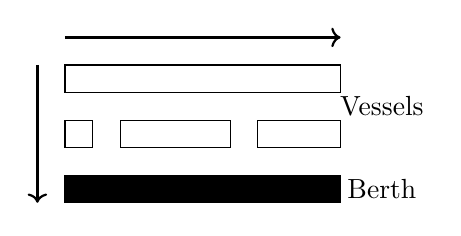
\begin{tikzpicture}[scale=0.35]
			\draw[rotate=90,fill=black] (0,0) rectangle (1,10);
			\draw[rotate=90](2,0) rectangle (3,3);
			\draw[rotate=90](2,4) rectangle (3,8);
			\draw[rotate=90](2,9) rectangle (3,10);
			\draw[rotate=90](4,0) rectangle (5,10);

			\draw[thick,->] (-11,5)--(-11,0);
			\draw[thick,->] (-10,6)--(0,6);

			\node at (1.5,0.5) {Berth};
			\node at (1.5,3.5) {Vessels};
		\end{tikzpicture}}
	\caption{Example of berth allocation. Vessels are docked in berth locations (horizontal) and are queued over time (vertical), and move in the directions indicated by the arrows.}
		\label{subfig:bapexample}
	\end{subfigure}

	\begin{subfigure}[b]{0.45\textwidth}
		\centerline{
		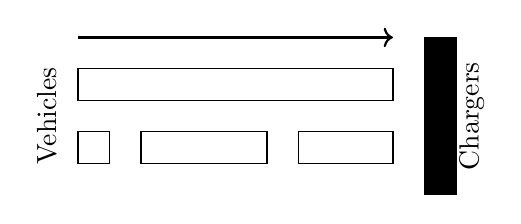
\begin{tikzpicture}[scale=0.4]
			\draw[fill=black] (0,0) rectangle (1,5);

			\draw[rotate=90](1,1) rectangle (2,4);
			\draw[rotate=90](1,5) rectangle (2,9);
			\draw[rotate=90](1,10) rectangle (2,11);
			\draw[rotate=90](3,1) rectangle (4,11);

			\draw[thick,->] (-11,5)--(-1,5);

			\node[rotate=90] at (-12,2.5) {Vehicles};
			\node[rotate=90] at (1.5,2.5) {Chargers};
		\end{tikzpicture}}
	\caption{Example of position allocation. Vehicles are placed in queues to be charged and move in the direction indicated by the arrow.}
		\label{subfig:papexample}
	\end{subfigure}
\end{figure}

The remainder of the paper proceeds as follows: Section \ref{sec:positionallocationproblem} the BAP is introduces with a MILP formulation example. Section \ref{sec:problemformulation} constructs the PAP and introduces battery dynamics into the MILP, and Section \ref{sec:example} demonstrates an example of the PAP formulation and its ability to optimally assigning vehicles while considering battery dynamics and meeting scheduling constraints. The paper ends in Section \ref{sec:conclusion} with concluding remarks.

\begin{table*}[!t]
	\caption{Notation used throughout the paper}
	\label{tab:variables}
	\centering
	\begin{tabular}{l l l l}
		\toprule
		\textbf{Variable} & \textbf{Description} & \textbf{Variable} & \textbf{Description} \\
		\toprule
		\multicolumn{4}{l}{Input values} \\
			$A$           & Number of buses in use &
			$I$           & Final index                               \\
			$M$           & An arbitrary very large upper bound value &
			$N$           & Number of total visits                    \\
			$O$           & Bounding box for rectangle packing        &
			$\vmathbb{O}$ & Set of rectangles to be packed in \(O\)   \\
			$Q$           & Number of chargers                        &
			$S$           & Length of charger                         \\
			$T$           & Time Horizon                              \\
		\hline
		\multicolumn{4}{l}{Input variables} \\
			$\Gamma_i$   & Array of visit id's                                             &
			$\alpha_i$   & Initial charge time for visit  $i$                              \\
			$\beta_{i}$  & Final charge for bus $i$ at the end of the time horizon         &
			$\epsilon_q$ & Cost of using charger $q$ per unit time                         \\
			$\gamma_i$   & Array of values indicating the next index visit $i$ will arrive &
			$\kappa_i$   & Battery capacity for bus \(i\)                                  \\
			$\lambda_i$  & Discharge of visit over route  $i$                              &
			$\nu$        & Minimum charge allowed on departure of visit \(i\)              \\
			$\tau_i$     & Time visit $i$ must leave the station                           &
			$\zeta_i$    & Discharge rate for vehicle \(i\)                                \\
			$a_i$        & Arrival time of visit  $i$                                      &
			$c_i$        & Detach time from charger for visit \(i\)                        \\
			$m_q$        & Cost of a visit being assigned to charger  $q$                  &
			$r_q$        & Charge rate of charger $q$ per unit time                        \\
			$s_q$        & Length of vehicle \(i\)                                         \\
		\hline
		\multicolumn{4}{l}{Decision Variables} \\
			$\delta_{ij}$ & If $v_i + s_i \leq v_j$ (\(\delta = 1\)) otherwise \(\delta = 0\)   &
			$\eta_i$      & Initial charge for visit $i$                                        \\
			$\sigma_{ij}$ & If \(u_i + p_i \leq u_j\) (\(\sigma = 1\)) otherwise \(\sigma = 0\) &
			$c_i$         & detach time from charger for visit $i$                              \\
			$g_i$         & Linearization term for bilinear terms $g_i := p_i w_{iq}$           &
			$p_i$         & Amount of time spent on charger for visit $i$                       \\
			$u_i$         & Initial charge time of visit $i$                                    &
			$v_i$         & Assigned queue for visit $i$                                        \\
			$w_{iq}$      & Vector representation of queue assignment                           \\
			\bottomrule
	\end{tabular}
\end{table*}

%%-------------------------------------------------------------------------------
% The Position Allocation Problem
\section{The Position Allocation Problem}
\label{sec:positionallocationproblem}
The BEB charge schedule formulation in this work builds upon the PAP. The PAP is a rectangle packing problem where a set of rectangles \(\vmathbb{O}\) are attempted to be optimally placed in a larger rectangle \(O\) as shown in Fig \ref{fig:packexample}. Both the set \(\vmathbb{O}\) and rectangle \(O\)'s width and height are used to represent quantifiable values. The rectangle packing problem is a NP-hard problem that can be used to describe many real life problems \cite{Bruin2013,Murata1995}. In some of these problems, the dimensions of \(\vmathbb{O}\) are held constant such as in the problem of packing modules on a chip, where the widths and height of the rectangles represent the physical width and heights of the modules \cite{Murata1995}. Other problems, such as the BAP, allow one or both sides of each rectangle to be decision variables \cite{Buhrkal2010}.

Within BAP, the set of rectangles (\(\vmathbb{O}\)) describe incoming vessels to be docked on a berth to be serviced and are to be packed into the rectangle (\(O\)) defined by the time horizon (\(T\)) and berth length (\(S\)) \cite{Dai2008}, as shown in Fig \ref{subfig:bapexample}. The BAP is commonly formed as a MILP \cite{Frojan2015,Buhrkal2010}. The PAP formulation utilizes the BAP to help determine which queue the bus should be placed on to be charged without violating time or space constraints \cite{Qarebagh2019}. Notation is summarized in Table \ref{tab:variables}.

\begin{figure}
	\centerline{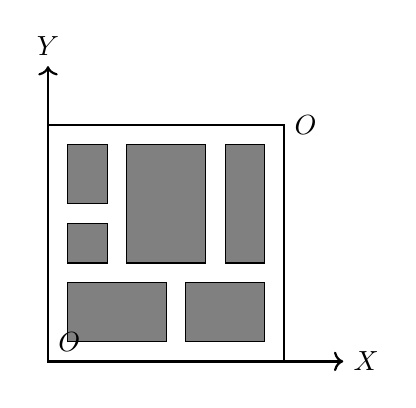
\begin{tikzpicture}[scale=0.25]
	    \draw [thick, -] (0,0) rectangle (12,12) node[right]{$O$};
	    \draw[fill=gray] (1,1) rectangle (6,4);
	    \draw[fill=gray] (11,11) rectangle (9,5);
	    \draw[fill=gray] (8,11) rectangle (4,5);
	    \draw[fill=gray] (1,11) rectangle (3,8);
	    \draw[fill=gray] (1,7) rectangle (3,5);
	    \draw[fill=gray] (11,1) rectangle (7,4);
        \draw [thick,<->] (0,15) node[above]{$Y$}                      --
                                 (0,0)node[above right]{$\vmathbb{O}$} --
                                 (15,0) node[right]{$X$};
	\end{tikzpicture}}
	\caption{Example of rectangle packing problem}
	\label{fig:packexample}
\end{figure}

The BAP solves the problem of optimally assigning incoming vessels to berth positions to be serviced (Fig \ref{subfig:bapexample}). The width and height of \(O\) represent the berth length \(S\) and time horizon \(T\), respectively. Similarly, the width and height for \(\vmathbb{O}\) represent the time spent to service vessel $i$ and the space taken by docking vessel $i$, respectively. The vessel characteristics (length of the vessel, arrival time, handling time, desired departure time) are assumed to be known for all $N$ vessels to be serviced. A representation of a BAP solution is shown in Fig \ref{fig:bap}.

The BAP objective is generally represented as minimizing some operational time for a given vessel \(i\). The operational time may be chosen to minimize time of arrival to time of departure, time spent being serviced, or overall waiting time (i.e. \(a_i \leq u_i\)) \cite{Voss2007, Buhrkal2010,Frojan2015}. The model must then constrain the vessel placement as to not allow overlap in time or space as well as disallowing discontinuities in arrival times to departure times.

The BAP formulation forms the basis of the PAP; however there are some slight differences in the way the variables are perceived. Starting service time (\(u\)) is now the starting charge time, the berth location (\(v\)) is now the queue for charger \(q\), and the service time (\(p\)) is now the time to charge. The following MILP describes the stated objective and constraints. The MILP is also shown in its entirety as it forms the foundation from which the PAP is constructed \cite{Qarebagh2019}.

\begin{figure}
	\centerline{
	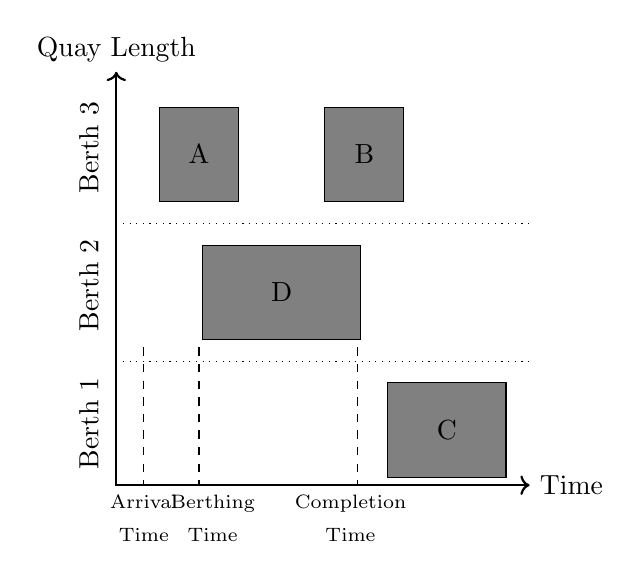
\begin{tikzpicture}[scale=0.35]
        \draw [thick,<->] (0,15) node[above]{Quay Length} --
                                 (0,0)                    --
                                 (15,0) node[right]{Time};
        \node[rectangle, draw, fill=gray, minimum width=1cm, minimum height = 1.2cm] at (3,12) {A};
        \node[rectangle, draw, fill=gray, minimum width=1cm, minimum height = 1.2cm] at (9,12) {B};
        \node[rectangle, draw, fill=gray, minimum width=2cm, minimum height = 1.2cm] at (6,7) {D};
        \node[rectangle, draw, fill=gray, minimum width=1.5cm, minimum height = 1.2cm] at (12,2) {C};

	\node [below,align=center] at (1.0,0) {\scriptsize Arrival\\ \scriptsize Time};
	\draw[dashed] (1.0,5)--(1.0,0);

	\node [below, align=center] at (3.5,0) {\scriptsize Berthing\\ \scriptsize Time};
	\draw[dashed] (3,5)--(3,0);

	\node [below, align=center] at (8.5,0) {\scriptsize Completion\\ \scriptsize Time};
	\draw[dashed] (8.75,5)--(8.75,0);

        \draw[dotted] (0, 4.5) -- (15, 4.5);
        \draw[dotted] (0, 9.5) -- (15, 9.5);

	\node[rotate=90] at (-1, 2.25) {Berth 1};
	\node[rotate=90] at (-1, 7.25) {Berth 2};
	\node[rotate=90] at (-1, 12.25) {Berth 3};

	\end{tikzpicture}
    }
	\caption{The representation of the berth-time space}
	\label{fig:bap}
\end{figure}

\begin{equation}
	\label{eq:bapobjective}
	min\; \sum_{i=1}^N (c_i - a_i)
\end{equation}

Subject to the following constraints:

\begin{subequations}
\label{eq:bapconstrs}
\begin{align}
    u_j - u_i - p_i - (\sigma_{ij} - 1)T \geq 0                     \label{subeq:baptime}         \\
    v_j - v_i - s_i - (\delta_{ij} - 1)S \geq 0                     \label{subeq:bapspace}        \\
    \sigma_{ij} + \sigma_{ji} + \delta_{ij} + \delta_{ji} \geq 1    \label{subeq:bapvalid_pos}    \\
    \sigma_{ij} + \sigma_{ji} \leq 1                                \label{subeq:bapsigma}        \\
    \delta_{ij} + \delta_{ji} \leq 1                                \label{subeq:bapdelta}        \\
    p_i + u_i = c_i                                                 \label{subeq:bapdetach}       \\
    a_i \leq u_i \leq (T - p_i)                                     \label{subeq:bapvalid_starts} \\
    \sigma_{ij} \in \{0,1\},\;\delta_{ij} \in \{0,1\}               \label{subeq:bapsdspace}
\end{align}
\end{subequations}

\noindent
Where, for this problem, the following are constants

\begin{itemize}
	\item \(S\)   : charger length
	\item \(T\)   : time horizon
	\item \(N\)   : number of incoming vehicles
	\item \(p_i\) : charging time for vehicle \(i\;; \forall 1 \leq i \leq N\)
	\item \(s_i\) : size of vehicle \(i\;; \forall 1 \leq i \leq N\)
	\item \(a_i\) : arrival time of vehicle \(i\;; \forall 1 \leq i \leq N\)
\end{itemize}

\noindent
and the following are decision variables

\begin{itemize}
    \item \(u_i\)         : starting time of service for vehicle \(i\;; \forall 1 \leq i \leq N\)
    \item \(v_i\)         : charger queue \(i\;; \forall 1 \leq i \leq N\)
    \item \(c_i\)         : departure time for vehicle \(i\;; \forall 1 \leq i \leq N\)
    \item \(\sigma_{ij}\) : \(u_i < u_j\;; \forall 1 \leq i < j \leq N\)
    \item \(\delta_{ij}\) : \(v_i < v_j\;; \forall 1 \leq i < j \leq N\)
\end{itemize}

The objective function \eqref{eq:bapobjective} minimizes the time spent to service each vehicle by minimizing over the difference between the departure time (\(c\)) and arrival time (\(a\)).

Constraints \ref{subeq:baptime}-\ref{subeq:bapdelta} are the ``queuing constraints". They are used to prevent overlapping in both space and time as shown in Fig \ref{fig:multipleassign}. In terms of the BAP, constraint \eqref{subeq:baptime} states that the starting service time (\(u\)) for vessel \(j\) must be greater than the starting time of vessel \(i\) plus its service time (\(p\)). The last term utilizes the Big-M notation to activate or deactivate the constraint. Specifically, \eqref{subeq:baptime} is active if both \(i\) and \(j\) are to visit the same queue (\(v_i = v_j\)). A value of \(\sigma_{ij} = 1\) will activate the constraint to ensure that \(i\) is complete before \(j\) is allowed to begin being serviced. If \(\sigma = 0\), then the constraint is of the form \(T + u_j + p_j > u_i\) rendering the constraint ``inactive" because \(u_i\) cannot be larger than \(T + u_j + p_j\).

In a similar fashion, \(\delta_{ij}\) effectively determines whether the vehicles will be charging at the same time (\(u_i + p_i \geq u_j\)). If \(\delta_{ij} = 1\) then \eqref{subeq:bapspace} is rendered active and vehicle \(i\) and \(j\) must be charging at the same time but in different queues.

Constraints \ref{subeq:bapvalid_pos}-\ref{subeq:bapdelta} are used to establish queuing by providing a relationship between queuing variables (\(u\) and \(v\)). Constraint \eqref{subeq:bapdelta} states that one of the following is true for each vehicle pair: \(u_i + p_i < u_j\) (\(\sigma_{ij} = 1\)), \(u_j < u_i + p_i\) (\(\sigma_{ji} = 1\)), \(v_i + s_i < v_j\) (\(\delta_{ij} = 1\)), \(v_j < v_i + s_i\) (\(\delta_{ji} = 1\)). Constraints \eqref{subeq:bapsigma} and \eqref{subeq:bapdelta} enforce consistency, i.e. \(u_i + p_i < u_j\) and \(u_j < u_i + p_i\) cannot hold true simultaneously. In a similar manner, \(v_i + s_i < u_j\) and \(u_j < v_i + s_i\) cannot be true simultaneously. This enforces a relationship between vessels: either one is before the other temporally or they are in different queues.

The last constraints enforce continuity for each vessel. Constraint \eqref{subeq:bapdetach} states that the service start time (\(u\)) plus the time to service vessel \(i\) (\(p\)) must equal the departure time (\(c\)). Constraint \eqref{subeq:bapvalid_starts} enforces the arrival time (\(a\)) must be less than or equal to the service start time (\(u\)) which must also be less than or equal to the latest time the vessel may begin to be serviced to stay within the time horizon. Constraint \eqref{subeq:bapsdspace} defines the set of values \(\sigma\) and \(\delta\).

The PAP has characteristics that can be leveraged and others that must be addressed to fit the desired model. An example of a property that much be addressed is that each vessel \(i\;; \forall 1 \leq i \leq N\) is assumed to be a new (i.e. unique) visit. This  a problem for accounting for battery dynamics when busses revisit after completing a route. Each bus visit must then be associated with a specific bus ID. An example of a property that can be leveraged is, due to the nature of the BAP, little effort is required to convert the problem from serial berth docking to parallel charge queuing. The results may be vectorized to achieve this goal \cite{Qarebagh2019}. Furthermore, this formulation allows \(S\) and \(T\) to be continuous or discrete \cite{Frojan2015,Buhrkal2010}. Because of this flexibility, the berth is discretized to accommodate \(Q\) chargers while time is kept continuous as shown in Fig \ref{fig:bap}.

\begin{figure}
	\centerline{
	\begin{tikzpicture}[scale=0.35]
		\draw [thick,<->] (0,15) node[above]{Quay Length} --
					 (0,0)                    --
					 (15,0) node[right]{Time};

		\node[rectangle, draw, minimum width=1.5cm, minimum height = 2cm] at (5,8) {\(i\)};
		\node[rectangle, draw, minimum width=1cm, minimum height = 1cm] at (2,2) {\(j\)};
		\node[rectangle, draw, dashed, minimum width=1cm, minimum height = 1.2cm] at (5,12) {\(k_1\)};
		\node[rectangle, draw, dashed, minimum width=1cm, minimum height = 1.2cm] at (7,6) {\(k_3\)};
		\node[rectangle, draw, dashed, minimum width=1cm, minimum height = 1.2cm] at (4,2) {\(k_2\)};
	\end{tikzpicture}
	}
	\caption{Examples of different methods of overlapping. Space overlap: \(v_{k_1} < v_{i} + s_i \therefore \delta_{k_{1}i} = 0\). Time overlap \(u_{k_1} < u_{j} + p_j \therefore \sigma_{k_{2}j} = 0\). Both space and time overlap \(\sigma_{k_{3}i} = 0\) and \(\delta_{k_{3}j} = 0\).}
	\label{fig:multipleassign}
\end{figure}

%%-------------------------------------------------------------------------------
%
\section{Problem Formulation}
\label{sec:problemformulation}
The MILP is formulated with two sets of constraints: queuing constraints and battery dynamics constraints. This section will build off and modify the previous formulation (\eqref{eq:bapobjective} and \eqref{eq:bapconstrs}) and progressively construct the battery dynamic constraints to create the Position Allocation MILP. All notation is defined in Table \ref{tab:variables}.

\subsection{Queuing Constraints}
\noindent
Consider the following set of constraints:

\begin{subequations}
\label{eq:packconstrs}
\begin{align}
    u_i - u_j - p_j - (\sigma_{ij} - 1)T \geq 0                      \label{subeq:time}         \\
    v_i - v_j - s_j - (\delta_{ij} - 1)Q \geq 0                      \label{subeq:space}        \\
    \sigma_{ij} + \sigma_{ji} + \delta_{ij} + \delta_{ji} \geq 1     \label{subeq:valid_pos}    \\
    \sigma_{ij} + \sigma_{ji} \leq 1                                 \label{subeq:sigma}        \\
    \delta_{ij} + \delta_{ji} \leq 1                                 \label{subeq:delta}        \\
    p_i + u_i = c_i                                                  \label{subeq:detach}       \\
    a_i \leq u_i \leq (T - p_i)                                      \label{subeq:valid_starts} \\
    c_i \leq \tau_i                                                  \label{subeq:valid_depart} \\
    \sigma_{ij} \in \{0,1\},\;\delta_{ij} \in \{0,1\}                \label{subeq:sdspace}      \\
    v_i \in \{1,2, ... , Q\}                                         \label{subeq:vspace}        \\
\end{align}
\end{subequations}

Constraints \eqref{subeq:time}-\eqref{subeq:valid_starts} are the same as previously described in Section \ref{sec:positionallocationproblem}, except charging time (\(p\)) is now a decision variable. Additionally, starting charge time (\(u\)), charge duration (\(p\)), and detach time (\(c\)) are continuous and charging queue (\(v\)) is discrete as represented in \eqref{subeq:vspace}. Constraint \eqref{subeq:valid_depart} states that the ending charge time \((c\)) must be less than or equal to the required departure time from the station \(\tau\).

Using purely the constraints in \eqref{eq:packconstrs} with the objective in \eqref{eq:bapobjective} would results in \(c_i\) being chosen as small as possible by employing \(p_i = 0,\; u_i = c_i\). Thus, the vehicles would not charge. Furthermore, it does not encode any revisiting of the BEB to the charging station. To remedy this, battery dynamic constraints are introduced.

\subsection{Battery Dynamic Constraints}
The battery dynamic constraints are used to drive time spent on the charger (\(p\)) as well define initial, final, and intermediate bus charges for each visit \(i\). The initial and final bus charges are predefined and are represented by the equations \(\eta = \alpha \kappa\) and \(\eta = \beta \kappa\), respectively, where \(\alpha\) and \(\beta\) are percentages of the battery capacity. The intermediate charges must be determined at solve time. 

To accomplish such a task, each arrival \(i\) must be associated with a initial charge (\(\eta_i\)) which represents the charge received from the previous visit minus the discharge observed while on route; however, because the PAP assumes each arrival is unique, bus visits must be associated with a unique bus ID to appropriately initialize charges for each visit. This visit/ID pair is represented as vector denoted by \(\Gamma\) where the index represents visit \(i\) and the value is the ID. To propagate charges forward, another term \(\gamma\) is introduced to represent the next index bus \(i\) arrives. For example, assume \(A = 3\) buses, \(N = 5\) visits, and \(\Gamma = [1,2,3,1,2]\) (that is to say, bus 1 arrives at the same time or before 2, bus 2 arrives at the same time or before 3, etc.). This would imply \(\gamma = [3,4,-1,-1,-1]\), where 0-indexing is assumed and -1 represents no further visits for bus \(\Gamma_i\). Assuming proportional battery dynamics, the charge propagation is represented by:

\begin{subequations}
\begin{align*}
    \eta_{\gamma_i} = \eta_i + \sum_{q=1}^Q p_i w_{iq} r_q - \lambda_i \\
    w_{iq} \in \{0,1\}
\end{align*}
\end{subequations}

Where \(\eta_{\gamma_i}\) is the initial charge for the next visit for bus \(\Gamma_i\), \(\eta_i\) is the initial charge for bus \(\Gamma_i\) for the current visit, \(\sum_{q=1}^Q p_i w_{iq} r_q\) represents the the amount of charge given by \(q\), and \(\lambda_i\) is the amount of discharge accrued during the route (\(\lambda = \textit{Discharge Rate [KW]}\cdot\textit{Route Duration [hr]}\)).

Maximum and minimum values for the intermediate charges are to be placed to ensure the battery is not overcharged and to guarantee sufficient charge for subsequent visits, respectively. In a similar fashion, these upper and lower bounds can be represented as:

\begin{subequations}
\begin{align*}
    \eta_i + \sum_{q=1}^Q p_i w_{iq} r_q \leq \kappa_{\Gamma_i}                 \\
    \eta_i + \sum_{q=1}^Q p_i w_{iq} r_q - \lambda_i \geq \nu \kappa_{\Gamma_i} \\
    w_{iq} \in \{0,1\}
\end{align*}
\end{subequations}

Where the upper bound is the battery capacity (\(\kappa\)) and the lower bound is a percentage of the battery capacity (\(\nu \kappa\)). Although the bounds and battery propagation have been defined, the term \(p_i w_{iq}\) is recognized as a bilinear term (two decision variables being multiplied together) which is nonlinear \cite{Rodriguez2013}. A standard way of linearizing a bilinear term that contains a continuous (\(p\)) and integer (\(w\)) term by introducing an either/or constraint and utilizing Big-M notation \cite{Chen2010,Rodriguez2013}.

\begin{subequations}
\begin{align}
    p_i + (1 - w_{iq})M \geq g_{iq}                                           \label{subeq:repgpgret}       \\
    p_i \leq g_{iq}                                                           \label{subeq:repgples}        \\
    Mw_{iq} \geq g_{iq}                                                       \label{subeq:repgwgret}       \\
    0 \leq g_{iq}                                                             \label{subeq:repgwles}        \\
    w_{iq} \in \{0,1\}
\end{align}
\end{subequations}

Where \(g_{iq} := p_i w_{iq}\) and \(M\) is defined sufficiently large such that for constraints \eqref{subeq:repgpgret} and \eqref{subeq:repgples} if \(w_{iq} = 1\) then the two equations will take the form of \(p_i \leq g_{eq}\) and \(p_i \geq g_{iq}\) effectively stating \(p_i = g_{iq}\). If \(w_{iq} = 0\) then the two equations will take the form of \(p_i \leq g_{eq}\) and \(p_i \geq g_{iq} - M\) which deactivates the constraint. In a similar fashion, \eqref{subeq:repgwgret} and \eqref{subeq:repgwles} state if \(w_{iq} = 0\) then the constraints take the form \(0 \geq g_{iq}\) and \(0 \leq g_{iq}\) directly implying \(0 = g_{iq}\). If \(w_{iq} = 1\) then the constraints take the form \(M \leq g_{iq}\) and \(0 \geq g_{iq}\) deactivating the constraint. Putting the two sets of constraints together defines the linearized representation of \(w_{iq} p_i\).

The last consideration is the objective function. The goal of the MILP is to utilize slow chargers as much as possible. To encourage this, assignment cost \(m\) and usage cost \(\epsilon\) are given to each charger type. The cost for both the assignment and utilization of slow chargers is less than that of the fast chargers. This objective function is represented in \eqref{eq:objective} for the MILP:

\begin{equation}
\label{eq:objective}
    \sum_{i=1}^N \sum_{q=1}^Q \Big( w_i m_q + g_i \epsilon_q \Big) \\
\end{equation}

\noindent
Subject to the constraints in \eqref{eq:packconstrs} as well as the following constraints for battery charger dynamics:

\begin{subequations}
\label{eq:dynconstrs}
\begin{align}
    \eta_i = \alpha \kappa_{\Gamma_i}                                         \label{subeq:init_charge}  \\
    \eta_i + \sum_{q=1}^Q g_{iq} r_q - \lambda_i = \eta_{\gamma_i}            \label{subeq:next_charge}  \\
    \eta_i + \sum_{q=1}^Q g_{iq} r_q - \lambda_i \geq \nu \kappa_{\Gamma_i}   \label{subeq:min_charge}   \\
    \eta_i + \sum_{q=1}^Q g_{iq} r_q \leq \kappa_{\Gamma_i}                   \label{subeq:max_charge}   \\
    \eta_i \geq \beta \kappa_{\Gamma_i}                                       \label{subeq:final_charge} \\
    p_i + (1 - w_{iq})M \geq g_{iq}                                           \label{subeq:gpgret}       \\
    p_i \leq g_{iq}                                                           \label{subeq:gples}        \\
    Mw_{iq} \geq g_{iq}                                                       \label{subeq:gwgret}       \\
    0 \leq g_{iq}                                                             \label{subeq:gwles}        \\
    \sum_{q=1}^Q qw_{iq} = v_i                                                \label{subeq:wmax}         \\
    \sum_{q=1}^Q w_{iq} = 1                                                   \label{subeq:wone}         \\
    w_{iq} \in \{0,1\}                                                        \label{subeq:wspace}
\end{align}
\end{subequations}

Constraints \eqref{subeq:init_charge}-\eqref{subeq:final_charge} provide initialization and terminal conditions as well as intermediate constraints to provide continuity in vehicle charges. Constraint \eqref{subeq:init_charge} states the first arrival for each bus is initialized with a charge of (\(\alpha \kappa_{\Gamma_i}\)). Constraint \eqref{subeq:next_charge} defines that the previous charge (\(\eta\)) plus the charging done by charger (\(q\)) minus the discharge amount due to completing route (\(\lambda\)). Constraints \eqref{subeq:min_charge} is similar to \eqref{subeq:next_charge}, except it states that the initial charge (\(\eta\)) plus the charge from (\(q\)) and the discharge from route (\(\lambda\)) must be greater than some percentage of its capacity (\(\kappa\)) in order to guarantee sufficient charge to complete the next route. Constraint \eqref{subeq:max_charge} states that the charging done for visit \(i\) cannot be greater than the capacity of the battery (\(\kappa\)). Constraint \eqref{subeq:final_charge} states that the last visit for each vehicle must have a minimum charge of (\(\beta \kappa_{\Gamma_i}\)). Constraint \eqref{subeq:final_charge} is included to guarantee a minimum initial charge for the next working day.

The constraints \eqref{subeq:gples}-\eqref{subeq:gwles} represent linearization of the bilinear term the \(g_{iq} := p_i w_{iq}\). The set of constraints \eqref{subeq:wmax}-\eqref{subeq:wone} define the linking constraint between the queuing constraint \(v\) and \(w\) (i.e \(1w_{i1} + 2w_{i2} + \cdots + Qw_{iQ} = v_i\)) and enforces that only a single \(w\) may be selected per visit, respectively. The last constraint \eqref{subeq:wspace} defines the set of values for \(w\).

%================================================================================
% Example
\section{Example}
\label{sec:example}

An example will now be presented to demonstrate the utility of the developed MILP. A description of the scenario is first presented followed by results.

\subsection{Scenario}
The given exampled utilizes \(A = 40\) buses with \(N = 220\) returns to the station divided between the \(A\) buses. Each bus has a 388 KWh battery that is required to stay above 25\% charge (97 KWh) to maintain battery health, and the bus is assumed to start with 90\% charge (349 KWh). Additionally, each bus is required to end with a minimum charge of 95\% (349 KWh). Planning is done over a 24 hour time horizon. \(Q = 9\) chargers are utilized where five of the chargers are slow charging (100 KWh) and four are fast charging (400 KWh). The slow chargers take longer, but are safer for the battery than the fast charger. Therefore, the slow chargers are modeled with a lower cost than than the fast charger for both assigning (\(m\)) and utilization (\(\epsilon\)) in the objective \eqref{eq:objective} as to penalize utilization of the fast chargers.

The bus schedules are randomly generated. It is assumed that each bus has no more than 30 minutes between route departures. Bus route durations are completely random. They may vary anywhere from the average time between the current and next arrival to the next arrival time (i.e. \(\frac{a_i + a_{\gamma_i}}{2}\) to \(a_{\gamma_i}\)). The discharge is assumed to be linear and is calculated via \(\lambda_i = rand(\frac{a_i + a_{\gamma_i}}{2},a_{\gamma_i})\zeta{\gamma_i}\) where \(1 \leq i \leq N\).

The optimization was performed using the Gurobi MILP solver \cite{Hespanha2018} on a machine running a quad-core Intel i7-9700 4.7 GHz processor. The optimizer was allowed to run for 20 minutes without finding the optimal solution. The following are the results that were obtained.

\subsection{Results}
The schedule generated by the MILP is shown in Fig \ref{fig:schedule}. The top graph indicates the slow charger usage, and the bottom indicates the fast charger usage. Although \(Q = 9\) chargers were used, Fig \ref{fig:schedule} shows that only five chargers were utilized. The MILP formalization will, in addition to utilizing the slow chargers as much as possible, use only the minimum required amount of chargers. This behavior is due to the rectangle packing constraints \eqref{eq:packconstrs}.

Each color in Fig \ref{fig:schedule} is used to identify a new bus visit. It is noted that the overlaps in Fig \ref{fig:schedule} indicate the waiting time of vehicle \(j\) whilst vehicle \(i\) charges. This is recognized by viewing the vertical bars. These bars indicate the time bus \(i\) is set to charge. The area before indicate waiting time and the area after indicates the time spent on the charger.

Fig \ref{fig:charges} depicts the charge for every bus over the time horizon. Every vehicle begins at 90\% charge, finishes at 95\% charge, and never goes below 25\% in the intermediate arrivals as stated in the constraints \eqref{eq:dynconstrs}. The total power used is summarized in Fig \ref{fig:usage} which is representative of the linear battery constraints modeled.

\begin{figure*}[ht]
	\centering
	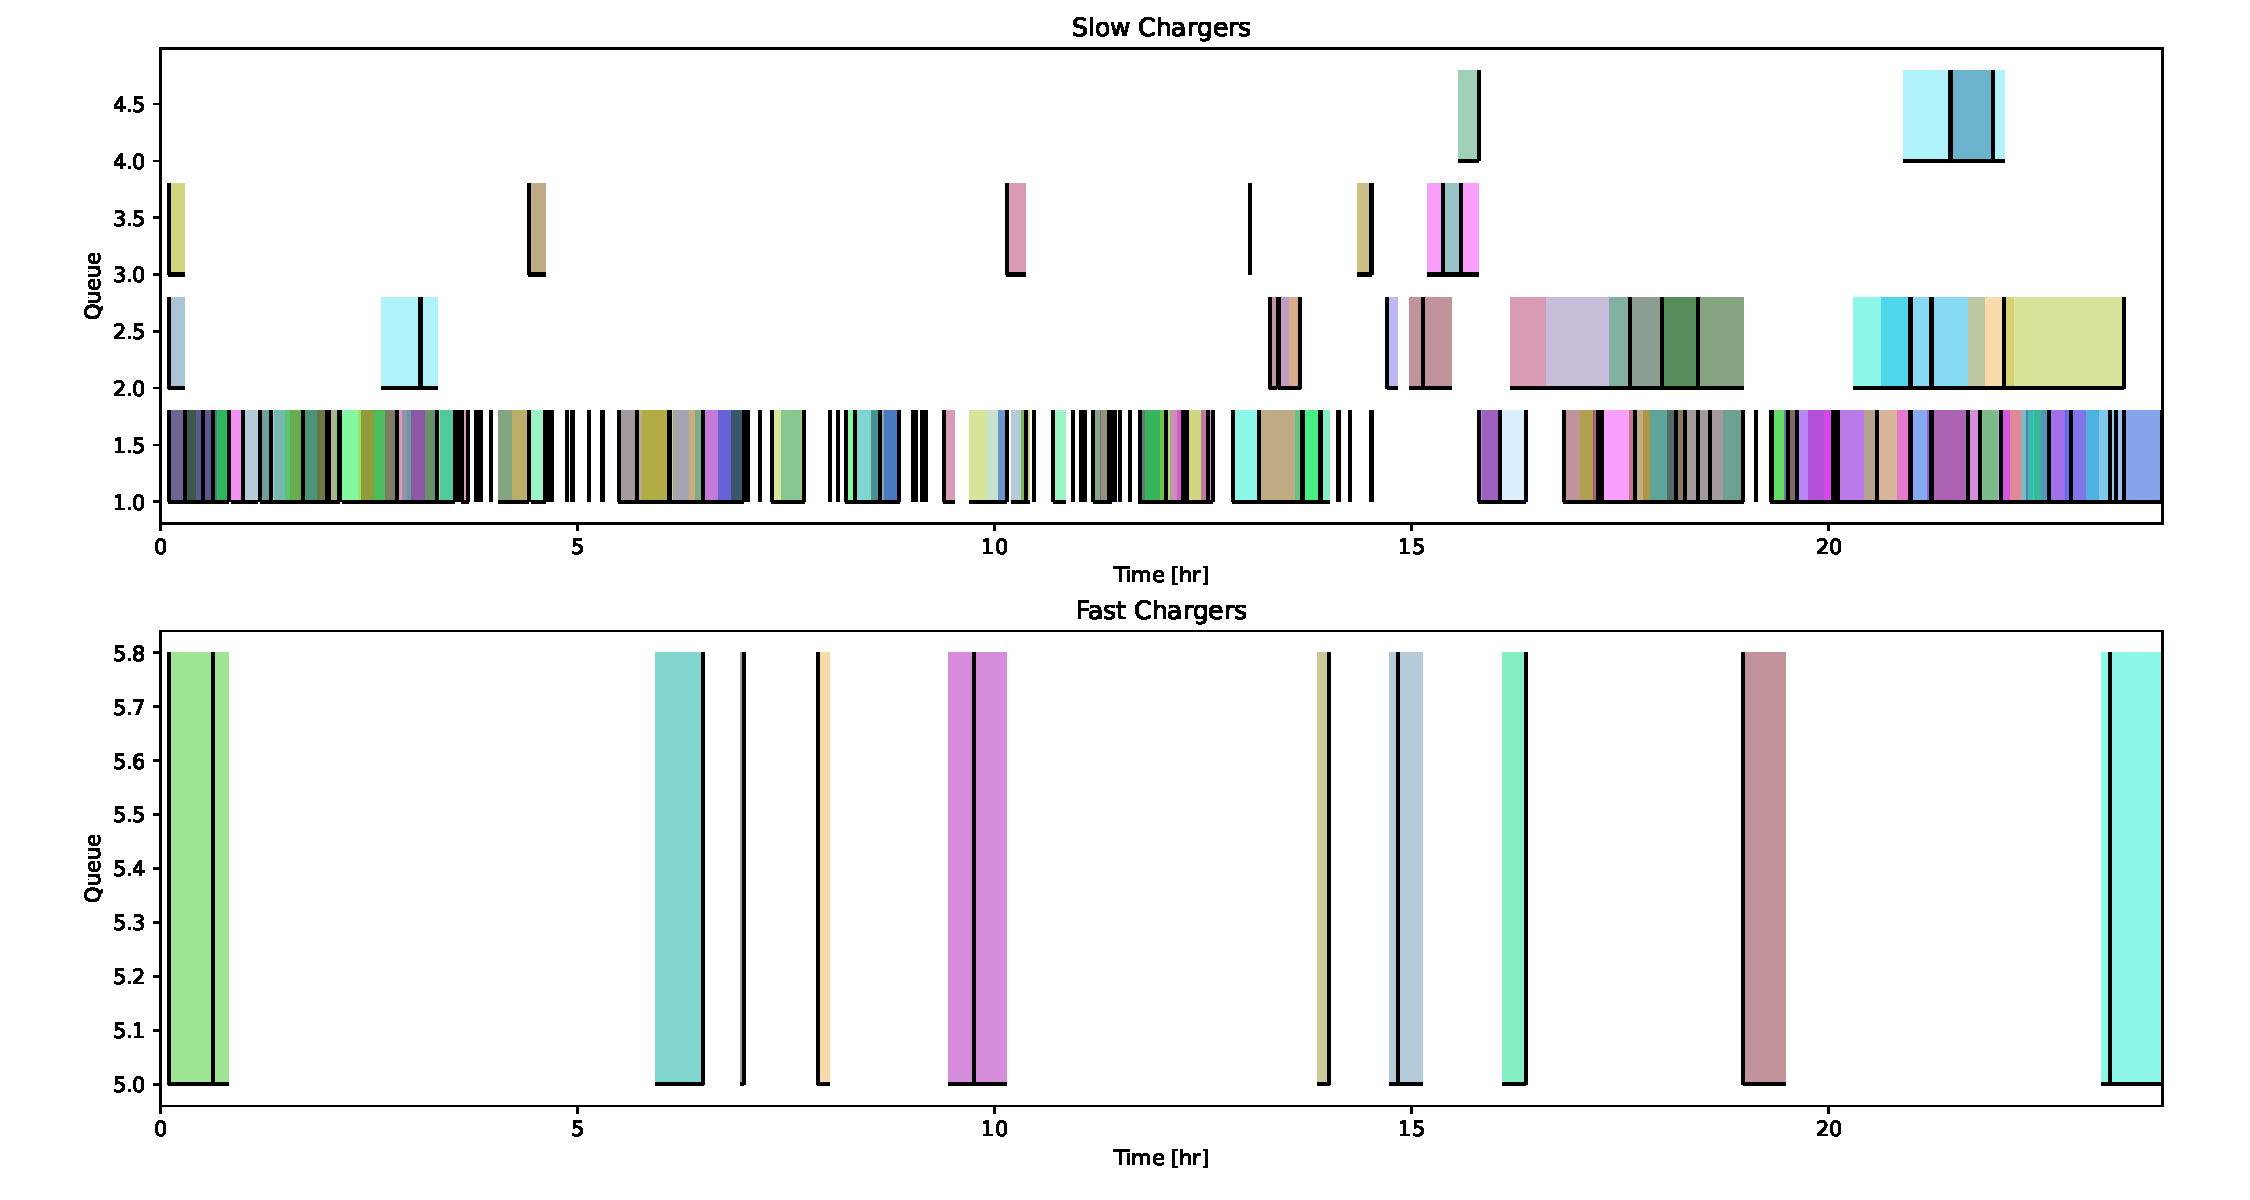
\includegraphics[trim=3in 0in 3in 0in, width=\linewidth, height=2.5in]{schedule.pdf}
	\caption{Bus schedule generated with PAP MILP. Each color indicates a new visit. The vertical bars indicate the time the vehicles are set to charge, the area before said bars indicate the waiting times for each visit \(1 \leq i \leq N\). Similarly, the area after the bars indicate the time spent on the charger.}
	\label{fig:charges}
\end{figure*}

\begin{figure}[ht]
	\centering
	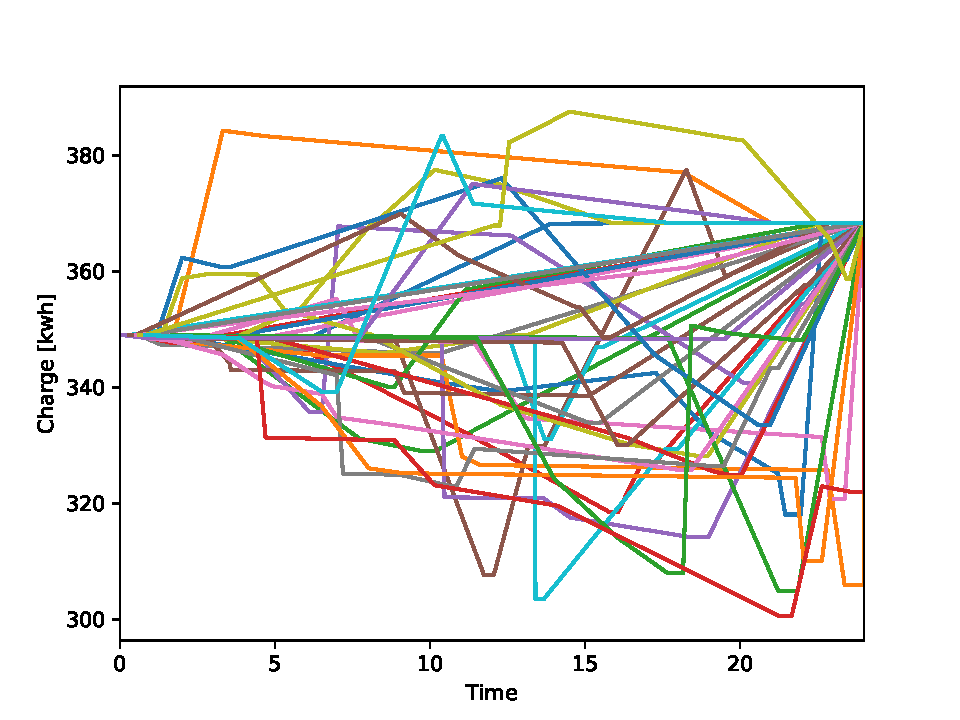
\includegraphics[trim=0in 0in 0in 0.75in, width=0.75\linewidth]{charges.pdf}
	\caption{Charges for each bus.}
	\label{fig:schedule}
\end{figure}


\begin{figure}[ht]
	\centering
	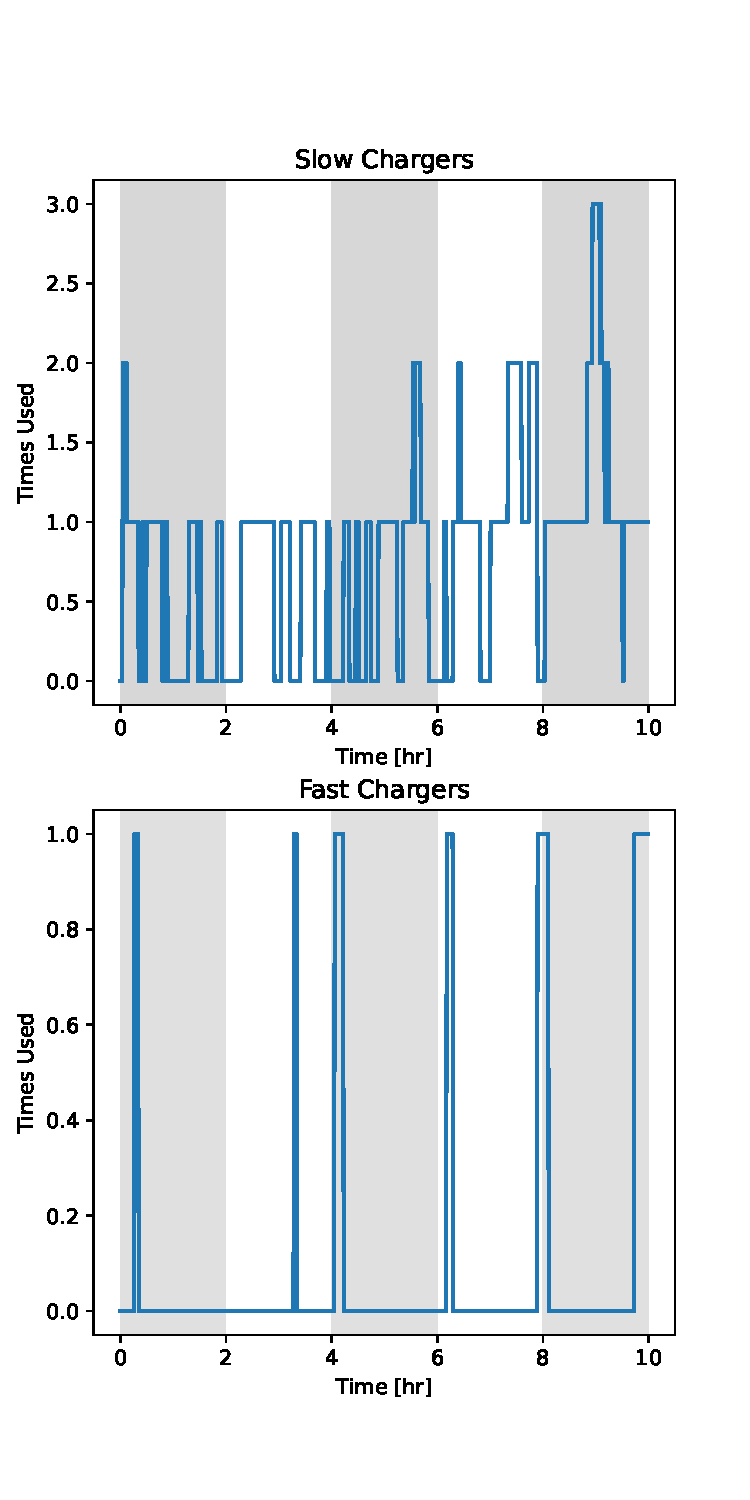
\includegraphics[trim=0in 0in 0in 0.5in, width=0.75\linewidth]{usage.pdf}
	\caption{Total power used.}
	\label{fig:usage}
\end{figure}

%%-------------------------------------------------------------------------------
% Conclusion
\section{Conclusion}
\label{sec:conclusion}
This work developed a MILP scheduling framework that optimally assigns slow and fast chargers to a BEB bus fleet assuming a constant schedule. The BAP was introduced with an example formulation and was then compared to the PAP. The PAP constructed on the BAP to allow the time spent on the charger (\(p\)) to be a decision variable. Because the original PAP required service time (\(p\)) to be given, linear battery dynamics were introduced to drive charging times. Additional constraints were also introduced to provide limits and continuity for the battery dynamics.

An example was presented that demonstrated the ability of the formulation to utilize slow chargers when possible and fast chargers when necessary. The example also demonstrated that if a surplus of chargers are given, the minimum amount of chargers will be utilized. This behavior is given by the packing constraints. The battery dynamic constraints to limit maximum and minimum charges was also observed. Future work may expand on this model by introducing first order battery dynamics to increase fidelity of the battery dynamic model.

%%================================================================================
% Bibliography
\bibliographystyle{IEEEtran}
\bibliography{main}

%%%%%%%%%%%%%%%%%%%%%%%%%%%%%%%%%%%%%%%%%%%%%%%%%%%%%%%%%%%%%%%%%%%%%%%%%%%%%%%%%
\end{document}
